% Created 2024-10-16 śro 21:35
% Intended LaTeX compiler: pdflatex
\documentclass[../main.tex]{subfiles}

% \usepackage[a4paper, margin=3cm]{geometry}
% \usepackage{amssymb} // not working

\usepackage[T1]{fontenc}
\usepackage[utf8]{inputenc}
\usepackage{graphicx}
\usepackage{longtable}
\usepackage{wrapfig}
\usepackage{rotating}
\usepackage[normalem]{ulem}
\usepackage{amsmath}
\usepackage{capt-of}
\usepackage{hyperref}
\usepackage{siunitx}
\usepackage{float}
\usepackage[polish]{babel}

\graphicspath{{../}}
\author{Wojciech Paderewski}
\date{\today}
\title{PCB}
\hypersetup{
 pdfauthor={Wojciech Paderewski},
 pdftitle={PCB},
 pdfkeywords={},
 pdfsubject={},
 pdflang={Polish}}

\begin{document}

Do zaprojektowania płytki drukowanej wykorzystano open-source'owy program KiCad. Zdecydowano się na zastosowanie dwustronnej płytki drukowanej.
Ostatecznie udało się uzyskać płytkę o wymiarach 138x53mm oraz szacowana wysokość wraz z komponentami na poziomie 1cm, 
co oznacza, że udało się osiągnąć cel wykonania jak najmniejszej płytki drukowanej.

W celu poprawy aspektów wizualnych płytki, zamówiona została pozłacana płyta drukowana. Uzyskano też pozłacaną ramkę, która powstała przez 
nie nakładanie soldermaski na krawędzie płytki, w taki sam sposób uzyskano pozłacane napisy. Płytka posiada 4 otwory montażowe ma śruby M3.
Otwory montażowe oraz otwory montażowe encodera są podłączone do masy, co pozwala na lepsze prowadzenie masy między warstwami płytki. W 
celu poprawy uzyskania jak najlepszego połączenia masy między warstwami, użyto dużo przelotek między warstwami. Zabieg ten pozwala na
lepsze ekranowanie ścieżek co powinno przyczynić się do zmniejszenia zakłóceń elektromagnetycznych. 

\begin{figure}[H]
    \centering
    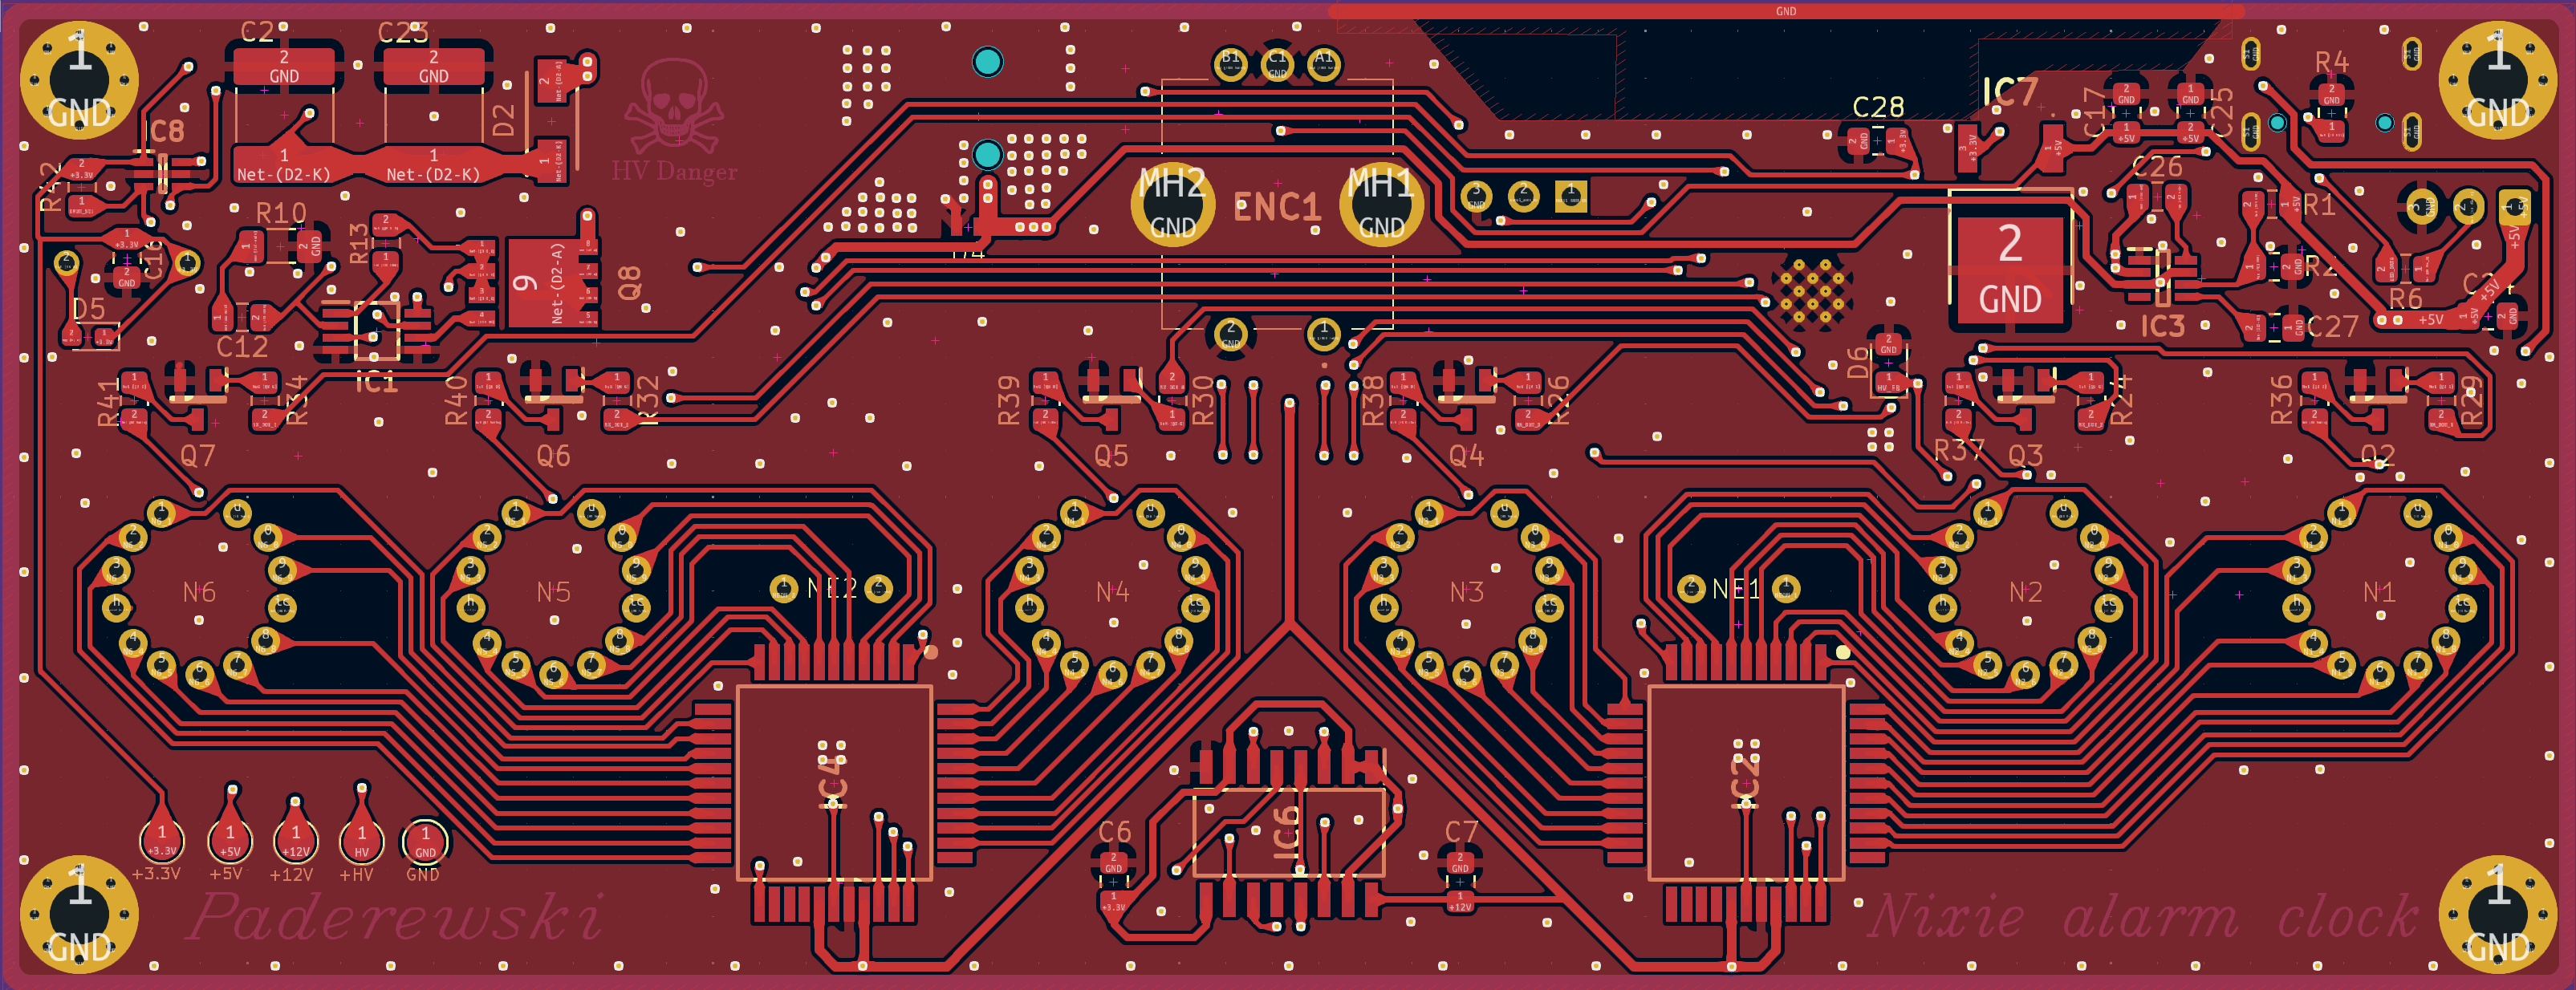
\includegraphics[width=1\textwidth]{TOP.png}
    \caption{Górna warstwa płytki drukowanej}
\end{figure}

\begin{figure}[H]
    \centering
    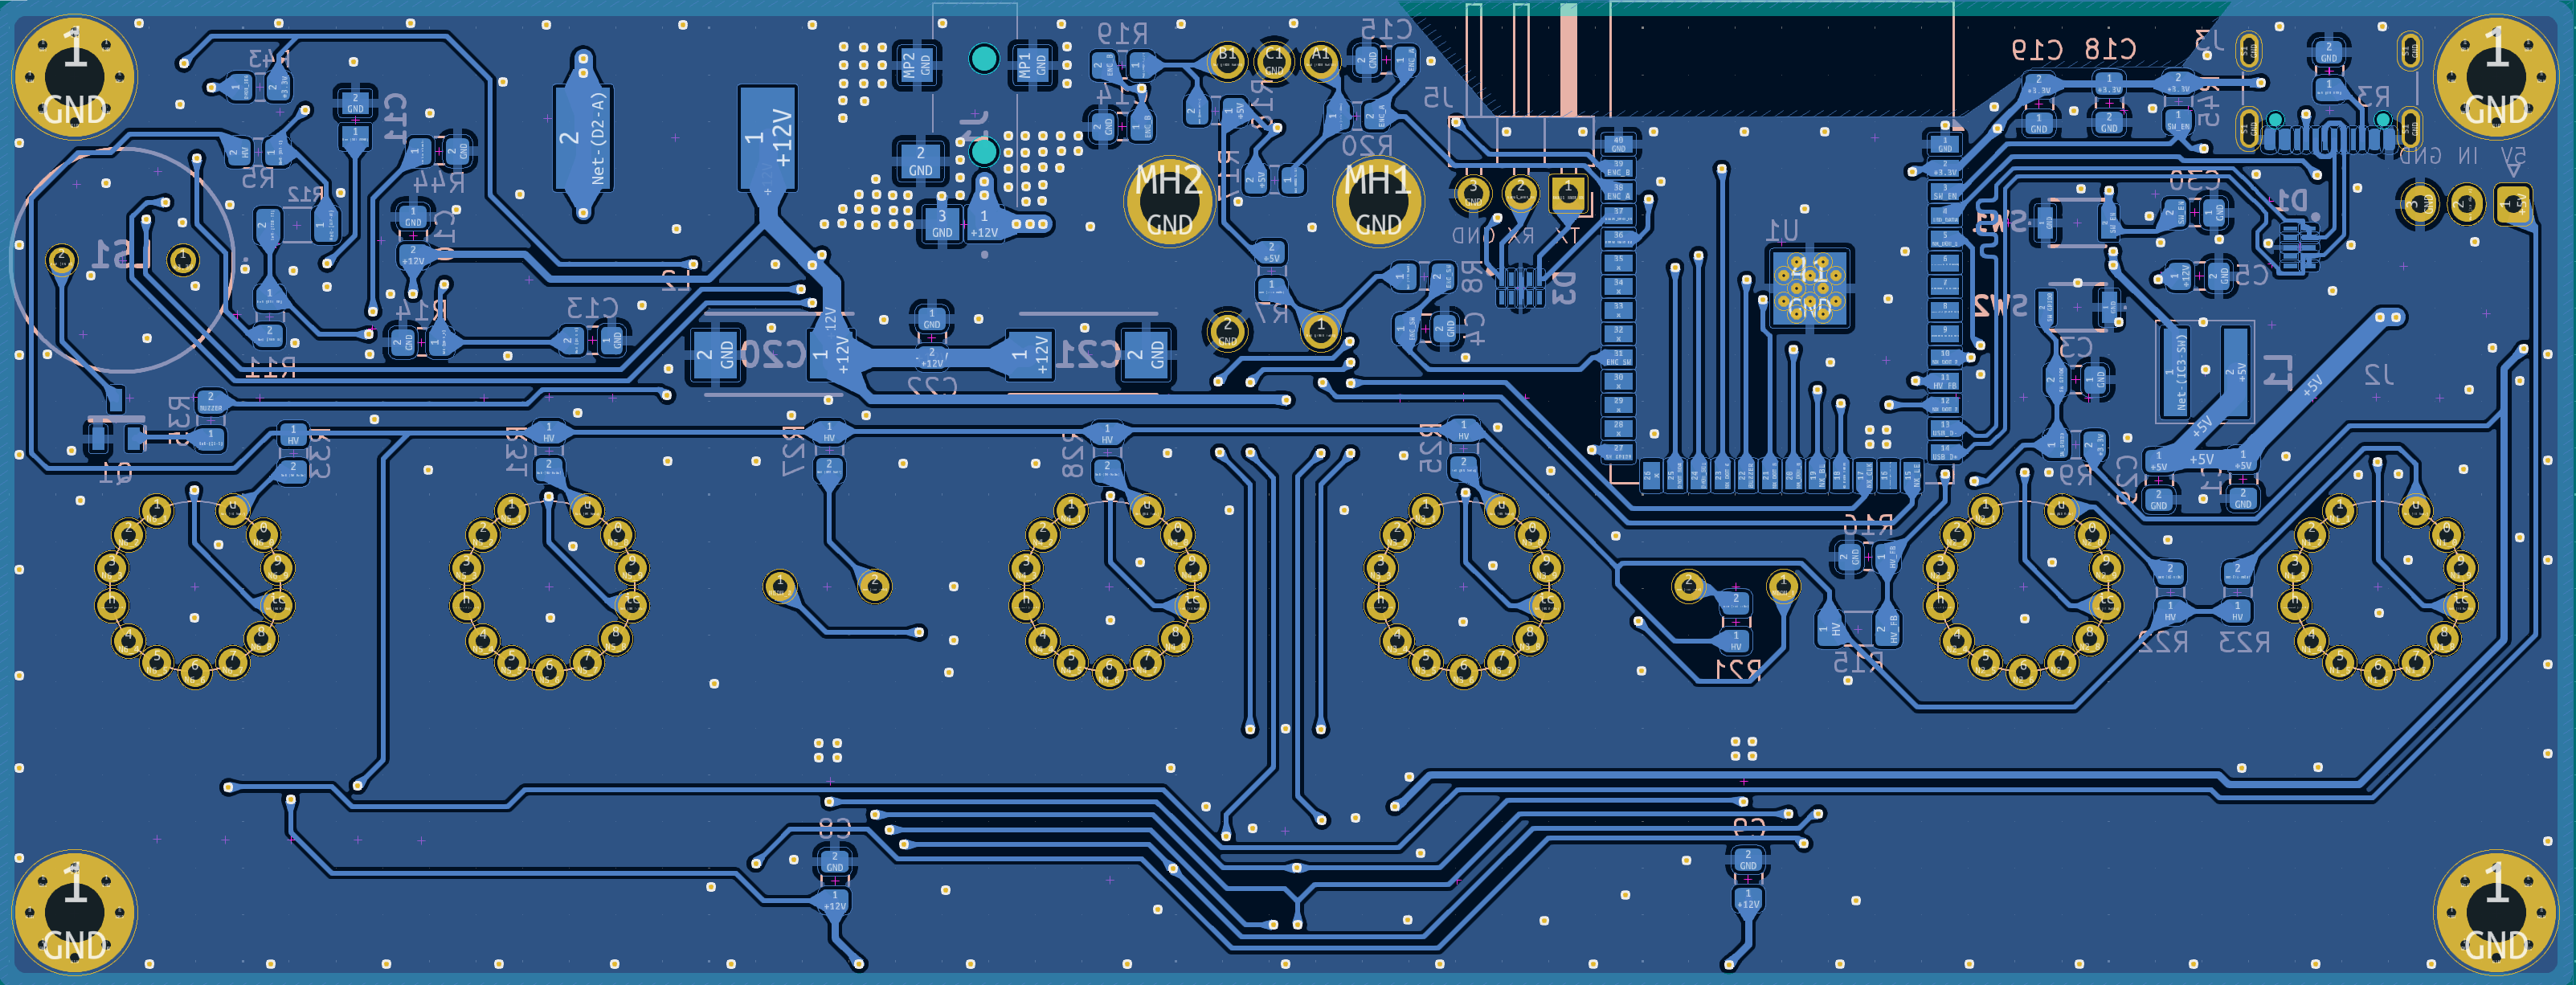
\includegraphics[width=1\textwidth]{BOTTOM.png}
    \caption{Dolna warstwa płytki drukowanej}
\end{figure}

\end{document}
